\chapter{基因组损伤与癌症}\label{ch:g11:cancer}

在显微镜下，健康肠道内壁的切片呈现出一种
有序的图景：\omterm{def:g10:cells-common-unit:cell}{细胞}排列成整齐的层次，每个\omterm{def:g10:cells-common-unit:cell}{细胞}的\omterm{def:g10:cells-common-unit:organelle}{细胞核}都不大，在层底分裂，
在层顶死亡，二者步调一致。同一切片中
相距仅几毫米处，一片\omterm{def:g10:cells-common-unit:cell}{细胞}却打乱了秩序：
\omterm{def:g10:cells-common-unit:cell}{细胞}拥挤、形状怪异，\omterm{def:g10:cells-common-unit:organelle}{细胞核}巨大而深染，随处分裂，
并向下方组织内侵入。这一片\omterm{def:g10:cells-common-unit:cell}{细胞}都源自
数年前的某一个\omterm{def:g10:cells-common-unit:cell}{细胞}；该\omterm{def:g10:cells-common-unit:cell}{细胞}获得了一次\omterm{def:g11:mutations:mutation}{突变}，使其
在不该分裂时仍然分裂，此后数年间又陆续积累了
数次\omterm{def:g11:mutations:mutation}{突变}。本章讨论\omterm{def:g11:cell-cycle-mitosis:cycle}{细胞周期}的调控如何失效、
是什么破坏了这些调控，以及事前与事后可以做些什么。

\section{不该分裂时却分裂}

\begin{definition}[癌症]\label{def:g11:cancer:cancer}
\emph{癌症}\index{癌症}是指这样一群\omterm{def:g10:cells-common-unit:cell}{细胞}，它们分裂时
不受正常\omterm{def:g10:cells-common-unit:cell}{细胞}分裂的调控约束，并
侵入周围组织。癌症始于一个\omterm{def:g10:cells-common-unit:cell}{细胞}，其
\omterm{def:g10:universal-dna:information}{DNA} 中调控\omterm{def:g11:cell-cycle-mitosis:cycle}{细胞周期}的
\omterm{def:g10:universal-dna:gene}{基因}积累了\omterm{def:g11:mutations:mutation}{突变}；该\omterm{def:g10:cells-common-unit:cell}{细胞}的后代形成\emph{肿瘤}\index{肿瘤}。
局限于原处的肿瘤称为\emph{良性}的；若其\omterm{def:g10:cells-common-unit:cell}{细胞}侵入
邻近组织，并经血液或淋巴转移到他处形成新的肿瘤（\emph{转移灶}），
则称为\emph{恶性}的。
\end{definition}

\begin{proposition}[癌症是一种基因组疾病]\label{prop:g11:cancer:genome}
\omterm{def:g11:cancer:cancer}{肿瘤}\omterm{def:g10:cells-common-unit:cell}{细胞}携带着同一个体其他\omterm{def:g10:cells-common-unit:cell}{细胞}所没有的\omterm{def:g11:mutations:mutation}{突变}：
这些是体\omterm{def:g10:cells-common-unit:cell}{细胞}\omterm{def:g11:mutations:mutation}{突变}，产生于某一个\omterm{def:g10:cells-common-unit:cell}{细胞}，并由其
后代遗传。\omterm{def:g11:cancer:cancer}{肿瘤}即为一个\emph{克隆}，并且会演化——
分裂更快或存活更好的\omterm{def:g10:cells-common-unit:cell}{细胞}会取而代之，此后的\omterm{def:g11:mutations:mutation}{突变}
又赋予其侵袭和扩散的能力。
\end{proposition}
\begin{proof}[证据]
对\omterm{def:g11:cancer:cancer}{肿瘤}\omterm{def:g10:cells-common-unit:cell}{细胞}与患者正常\omterm{def:g10:cells-common-unit:cell}{细胞}的 \omterm{def:g10:universal-dna:information}{DNA} 进行测序，
发现数以千计的差异，这些差异全部存在于\omterm{def:g11:cancer:cancer}{肿瘤}中，
健康组织中则没有；同样的少数几个\omterm{def:g10:universal-dna:gene}{基因}在每个
\omterm{def:g11:cancer:cancer}{肿瘤}中都发生了\omterm{def:g11:mutations:mutation}{突变}。在女性\omterm{def:g11:cancer:cancer}{肿瘤}\omterm{def:g10:cells-common-unit:cell}{细胞}中，失活的总是
两条 X \omterm{def:g11:cell-cycle-mitosis:chromosome}{染色体}中的同一条，这正是源自单一\omterm{def:g10:cells-common-unit:cell}{细胞}的特征。
\omterm{def:g11:mutations:mutagen}{诱变剂}即是\omterm{def:g11:cancer:carcinogen}{致癌物}：能够提高
\omterm{def:g11:mutations:mutation}{突变}率（见\cref{ch:g11:mutations}）的因素，同样会提高\omterm{def:g11:cancer:cancer}{癌症}发生率，
且往往有数十年的延迟。
\end{proof}

\begin{omfigure}
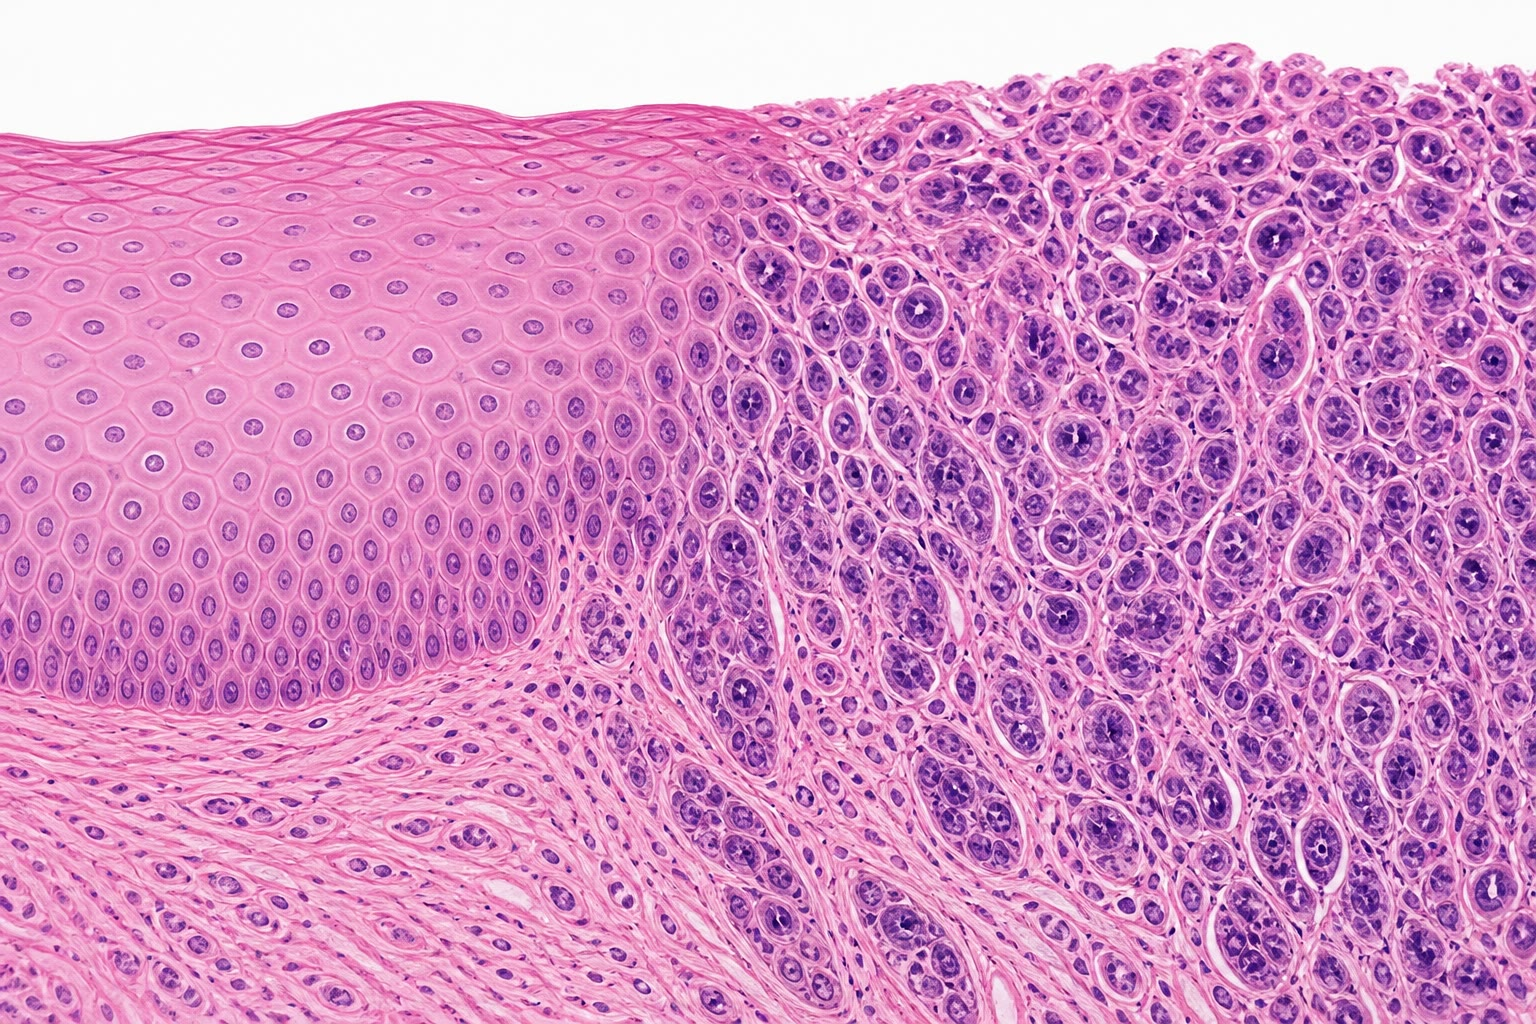
\includegraphics[width=0.62\linewidth]{images/book2/ai/g11-cancer-histology.jpg}

{\small 染色组织切片：左侧为有序排列的\omterm{def:g10:cells-common-unit:cell}{细胞}，
层次整齐；右侧为杂乱拥挤的\omterm{def:g10:cells-common-unit:cell}{细胞}团，\omterm{def:g10:cells-common-unit:organelle}{细胞核}大而
形状不规则，并向组织内侵入。两者之间的边界
即为\omterm{def:g11:cancer:cancer}{肿瘤}的边界。}
\end{omfigure}

\section{加速器与刹车}

\begin{proposition}[两类基因调控细胞周期]\label{prop:g11:cancer:genes}
\omterm{def:g10:cells-common-unit:cell}{细胞}是否分裂，取决于一类\omterm{def:g11:gene-expression:protein}{蛋白质}，它们的作用
如同车辆的油门与刹车。
\begin{itemize}
  \item \emph{原癌基因}\index{原癌基因}编码的\omterm{def:g11:gene-expression:protein}{蛋白质}
        在生长信号到达时，推动\omterm{def:g10:cells-common-unit:cell}{细胞}进入周期，
        这类\omterm{def:g11:gene-expression:protein}{蛋白质}包括生长信号的受体，以及把信号
        传递至\omterm{def:g10:cells-common-unit:organelle}{细胞核}的中继分子。若\omterm{def:g11:mutations:mutation}{突变}使此类
        \omterm{def:g11:gene-expression:protein}{蛋白质}持续处于活化状态，该\omterm{def:g10:universal-dna:gene}{基因}便转变为
        \emph{癌\omterm{def:g10:universal-dna:gene}{基因}}：油门被踩死。单个\omterm{def:g11:mutations:mutation}{突变}
        的\omterm{def:g10:universal-dna:gene}{等位基因}即已足够。
  \item \emph{抑癌基因}\index{抑癌基因}
        编码的\omterm{def:g11:gene-expression:protein}{蛋白质}使\omterm{def:g11:cell-cycle-mitosis:cycle}{细胞周期}停止，停止点位于
        S 期之前和\omterm{def:g11:cell-cycle-mitosis:cycle}{有丝分裂}之前的检验点，在 \omterm{def:g10:universal-dna:information}{DNA} 受损时，
        它们会触发修复，或在损伤无法修复时引发\omterm{def:g10:cells-common-unit:cell}{细胞}
        自我毁灭。使这类\omterm{def:g11:gene-expression:protein}{蛋白质}失活的\omterm{def:g11:mutations:mutation}{突变}，
        相当于去掉了一个刹车；\omterm{def:g10:cells-common-unit:cell}{细胞}有两个\omterm{def:g10:universal-dna:gene}{等位基因}，因此
        两者都必须丢失。
\end{itemize}
最为人熟知的抑癌蛋白是 p53，它在约半数
人类\omterm{def:g11:cancer:cancer}{癌症}中失活。
\end{proposition}
\admitted

\begin{omfigure}
\begin{tikzpicture}[font=\small, >=Stealth,
  b/.style={draw, rounded corners, align=center, text width=2.8cm, minimum height=1.0cm}]
  \node[b, fill=omMeth!15] (sig) at (0,1.2) {生长信号 \\来自其他细胞};
  \node[b, fill=omMeth!15] (onc) at (3.8,1.2) {原癌基因蛋白 \\传递信号};
  \node[b, fill=omDef!15] (cyc) at (7.6,1.2) {细胞进入 \\细胞周期};
  \node[b, fill=omDef!15] (div) at (11.4,1.2) {细胞分裂};
  \draw[->, thick] (sig) -- (onc); \draw[->, thick] (onc) -- (cyc); \draw[->, thick] (cyc) -- (div);
  \node[b, fill=omThm!12] (dam) at (3.8,-1.4) {检测到 \\DNA 损伤};
  \node[b, fill=omThm!12, text width=3.1cm] (p53) at (7.6,-1.4) {抑癌蛋白 \\（p53\dots）};
  \node[b, fill=omThm!12, text width=3.4cm] (halt) at (11.4,-1.4) {使细胞周期停止；\\修复，或自我毁灭};
  \draw[->, thick] (dam) -- (p53); \draw[->, thick] (p53) -- (halt);
  \draw[thick, omThm] (11.4,-0.85) -- (11.4,0.5);
  \draw[thick, omThm] (11.1,0.5) -- (11.7,0.5);
  \node[anchor=east, font=\scriptsize, omThm, align=right] at (11.0,-0.2) {刹车};
  \node[anchor=west, font=\scriptsize, omMeth!60!black] at (0.2,2.05) {油门};
\end{tikzpicture}

{\small \omterm{def:g10:cells-common-unit:cell}{细胞}分裂的调控。\omterm{prop:g11:cancer:genes}{原癌基因}蛋白传递生长信号，
并推动\omterm{def:g10:cells-common-unit:cell}{细胞}进入周期（油门）；抑癌蛋白
在 \omterm{def:g10:universal-dna:information}{DNA} 受损时使\omterm{def:g10:cells-common-unit:cell}{细胞}停止分裂（刹车）。癌\omterm{def:g10:universal-dna:gene}{基因}
是被卡在开启状态的油门；失去功能的\omterm{prop:g11:cancer:genes}{抑癌基因}，
则是被拆除的刹车。}
\end{omfigure}

\begin{example}[两个常见基因]\label{ex:g11:cancer:genes}
生长信号的受体位于许多\omterm{def:g10:cells-common-unit:cell}{细胞}的\omterm{def:g10:cells-common-unit:cell}{细胞}膜上；
该\omterm{def:g10:universal-dna:gene}{基因}中的一次替换，使受体在没有
任何外部信号时仍持续发出信号——这是一种在约三分之一的结肠癌与肺
癌中被发现的癌\omterm{def:g10:universal-dna:gene}{基因}。另一方面，p53 \omterm{def:g10:universal-dna:gene}{基因}
则以各种可能的方式发生\omterm{def:g11:mutations:mutation}{突变}而失活：替换使其
空间结构改变，缺失，以及过早出现的终止\omterm{def:g11:gene-expression:code}{密码子}。失去 p53 的\omterm{def:g10:cells-common-unit:cell}{细胞}
在复制 \omterm{def:g10:universal-dna:information}{DNA} 之前不会停下来修复，因此积累
\omterm{def:g11:mutations:mutation}{突变}的速度更快：失去这一刹车，会加速整个过程。
\end{example}

\section{数个步骤，多年积累}

\begin{proposition}[癌症是多步骤的过程]\label{prop:g11:cancer:multistep}
单个\omterm{def:g11:mutations:mutation}{突变}并不足以形成\omterm{def:g11:cancer:cancer}{癌症}。\omterm{def:g10:cells-common-unit:cell}{细胞}必须积累
若干\omterm{def:g11:mutations:mutation}{突变}——通常是一个癌\omterm{def:g10:universal-dna:gene}{基因}被激活，以及两个或更多\omterm{prop:g11:cancer:genes}{抑癌基因}失活——
并且每一次相继的\omterm{def:g11:mutations:mutation}{突变}，通过增强
克隆的增殖，增加了下一次\omterm{def:g11:mutations:mutation}{突变}
可能发生的\omterm{def:g10:cells-common-unit:cell}{细胞}数目。这一过程需要数年至数十年，因此
大多数\omterm{def:g11:cancer:cancer}{癌症}的发病率随年龄急剧上升，这也解释了为何
\omterm{def:g11:cancer:carcinogen}{致癌物}的作用往往在接触后二十或三十年才显现。
\end{proposition}
\begin{proof}[证据]
在结肠中可以观察到各个阶段：一个携带
一次\omterm{prop:g11:cancer:genes}{抑癌基因}\omterm{def:g11:mutations:mutation}{突变}的小型良性息肉；一个加入了癌\omterm{def:g10:universal-dna:gene}{基因}的较大息肉；以及一个
同时丢失 p53 的浸润性\omterm{def:g11:cancer:cancer}{肿瘤}。这一系列过程约包含四至
六次\omterm{def:g11:mutations:mutation}{突变}，历时十至二十年，每个阶段都能在下一阶段的\omterm{def:g10:cells-common-unit:cell}{细胞}中找到。
\omterm{def:g11:cancer:cancer}{癌症}发病率大致随年龄的五次方增长，
这正是约五到六个相互独立的罕见事件必须
全部发生于同一\omterm{def:g10:cells-common-unit:cell}{细胞}时所预期的曲线。遗传了\omterm{prop:g11:cancer:genes}{抑癌基因}
一个\omterm{def:g11:mutations:mutation}{突变}\omterm{def:g10:universal-dna:gene}{等位基因}的人，会更早、更频繁地
患上相应\omterm{def:g11:cancer:cancer}{癌症}，因为每个\omterm{def:g10:cells-common-unit:cell}{细胞}中已经完成了一步。
\end{proof}

\begin{omfigure}
\begin{tikzpicture}[font=\small, >=Stealth]
  \tikzset{c/.style={circle, draw, inner sep=0, minimum size=0.28cm}}
  % stage 1: one normal cell mutates
  \foreach \x in {0,0.35,...,1.05} \foreach \y in {0,0.35,0.7} \node[c, fill=omDef!15] at (\x,\y) {};
  \node[c, fill=omProp!60] at (0.7,0.35) {};
  \node[anchor=north, align=center, text width=2.4cm] at (0.5,-0.4) {一个细胞获得 \\ 突变 1};
  \draw[->, thick] (1.5,0.35) -- (2.3,0.35) node[midway, above, font=\scriptsize] {年};
  % stage 2: clone
  \begin{scope}[xshift=2.7cm]
    \foreach \x in {0,0.35,...,1.4} \foreach \y in {0,0.35,0.7} \node[c, fill=omDef!15] at (\x,\y) {};
    \foreach \x in {0.35,0.7,1.05} \foreach \y in {0.35,0.7} \node[c, fill=omProp!60] at (\x,\y) {};
    \node[c, fill=omThm!70] at (0.7,0.35) {};
    \node[anchor=north, align=center, text width=2.6cm] at (0.7,-0.4) {其克隆生长；\\ 一个细胞获得 \\ 突变 2};
  \end{scope}
  \draw[->, thick] (4.6,0.35) -- (5.4,0.35) node[midway, above, font=\scriptsize] {年};
  % stage 3: larger clone
  \begin{scope}[xshift=5.8cm]
    \foreach \x in {0,0.35,...,1.75} \foreach \y in {0,0.35,0.7,1.05} \node[c, fill=omProp!60] at (\x,\y) {};
    \foreach \x in {0.35,0.7,1.05,1.4} \foreach \y in {0.35,0.7} \node[c, fill=omThm!70] at (\x,\y) {};
    \node[c, fill=black!70] at (0.7,0.35) {};
    \node[anchor=north, align=center, text width=2.8cm] at (0.9,-0.4) {突变 3 出现于 \\ 最快克隆中：\\ 浸润性癌症};
  \end{scope}
  \draw[->, thick] (8.0,0.35) -- (8.8,0.35) node[midway, above, font=\scriptsize] {年};
  \begin{scope}[xshift=9.2cm]
    \foreach \x in {0,0.35,...,2.1} \foreach \y in {0,0.35,0.7,1.05} \node[c, fill=omThm!70] at (\x,\y) {};
    \foreach \x in {0.35,0.7,...,1.75} \foreach \y in {0.35,0.7} \node[c, fill=black!70] at (\x,\y) {};
    \node[anchor=north, align=center, text width=2.6cm] at (1.05,-0.4) {肿瘤：克隆的 \\ 克隆};
  \end{scope}
\end{tikzpicture}

{\small 克隆演化。每一次加快分裂的\omterm{def:g11:mutations:mutation}{突变}都会扩大
下一次\omterm{def:g11:mutations:mutation}{突变}可能发生的克隆；经过数次这样的
步骤、历经数年，某一谱系便失去了全部调控。\omterm{def:g11:cancer:cancer}{肿瘤}是一个
克隆的巢，最新的克隆位于较早的克隆之内。}
\end{omfigure}

\begin{omfigure}
\begin{tikzpicture}
\begin{axis}[
  width=0.86\linewidth, height=5.6cm,
  axis x line=bottom, axis y line=left,
  xmin=0, xmax=90, ymin=0, ymax=3200,
  xlabel={年龄（岁）}, ylabel={每年每 100\,000 人新发癌症数},
  xlabel style={font=\small, at={(axis description cs:0.5,-0.12)}, anchor=north},
  ylabel style={font=\small},
  tick label style={font=\small}, xtick={0,20,40,60,80}, ytick={0,1000,2000,3000},
]
\addplot[thick, omThm, mark=*, mark size=1.4pt] coordinates
  {(5,20) (15,25) (25,45) (35,110) (45,300) (55,700) (65,1500) (75,2400) (85,3000)};
\end{axis}
\end{tikzpicture}

{\small 所有\omterm{def:g11:cancer:cancer}{癌症}的年发病率随年龄的变化（数据取自各国登记机构，
已四舍五入）。增长远比正比快：从
35 岁到 70 岁，年龄翻了一倍，发病率却升高了二十倍，
这正是若干罕见事件必须全部发生于同一\omterm{def:g10:cells-common-unit:cell}{细胞}的特征。}
\end{omfigure}

\section{损害基因组的因素}

\begin{definition}[致癌物]\label{def:g11:cancer:carcinogen}
\emph{致癌物}\index{致癌物}是指能够提高
\omterm{def:g11:cancer:cancer}{癌症}风险的因子。大多数是\omterm{def:g11:mutations:mutagen}{诱变剂}：阳光中的紫外线（皮肤癌）、
烟草烟雾中的焦油（肺癌、口腔癌、膀胱癌）、电离辐射、
石棉纤维、酒精、某些霉菌。另有一些以其他方式起作用：
某些病毒携带的\omterm{def:g10:universal-dna:gene}{基因}会干扰\omterm{def:g10:cells-common-unit:cell}{细胞}的“刹车”——人乳头瘤
病毒几乎导致所有宫颈癌，肝炎病毒导致许多肝癌——而慢性
炎症，以及使组织持续分裂的激素，会增加
在其中可能发生\omterm{def:g11:mutations:mutation}{突变}的
分裂次数。
\end{definition}

\begin{omfigure}
\begin{tikzpicture}
\begin{axis}[
  width=0.86\linewidth, height=5.4cm,
  axis x line=bottom, axis y line=left,
  xmin=0, xmax=45, ymin=0, ymax=30,
  xlabel={每日吸烟支数}, ylabel={肺癌相对风险},
  xlabel style={font=\small, at={(axis description cs:0.5,-0.12)}, anchor=north},
  ylabel style={font=\small},
  tick label style={font=\small}, xtick={0,10,20,30,40}, ytick={0,5,10,15,20,25,30},
]
\addplot[thick, omThm, mark=*, mark size=1.5pt] coordinates
  {(0,1) (5,6) (10,10) (15,14) (20,17) (25,20) (30,22) (40,25)};
\end{axis}
\end{tikzpicture}

{\small 以不吸烟者为基准的肺癌相对风险，与数十年间
每日吸烟支数的关系（取自长期研究，
已取整）。风险随剂量上升，这正是\omterm{def:g11:mutations:mutagen}{诱变剂}作用于肺部的
预期结果。}
\end{omfigure}

\begin{example}[烟草]\label{ex:g11:cancer:tobacco}
烟雾中约含七十种\omterm{def:g11:cancer:carcinogen}{致癌物}；苯并芘一旦被
\omterm{def:g10:cells-common-unit:cell}{细胞}自身的酶活化，便会与鸟嘌呤结合，
并在这些位置上引起替换。吸烟者肺部\omterm{def:g11:cancer:cancer}{肿瘤}中的p53基因通常
恰好带有这样的替换，其位置正是苯并芘
最易结合的几处之一——\omterm{def:g11:mutations:mutagen}{诱变剂}在
序列中留下了特征“印记”。在香烟出现之前，肺癌十分罕见；吸烟
导致十分之九的肺癌，戒烟后十年内风险可减半，
因为携带早期\omterm{def:g11:mutations:mutation}{突变}的\omterm{def:g10:cells-common-unit:cell}{细胞}会逐步
被取代。
\end{example}

\begin{proposition}[遗传易感性]\label{prop:g11:cancer:inherited}
\omterm{def:g11:cancer:cancer}{癌症}本身并不遗传——它是体\omterm{def:g10:cells-common-unit:cell}{细胞}
\omterm{def:g11:mutations:mutation}{突变}所致的疾病——但\omterm{prop:g11:cancer:genes}{抑癌基因}的\omterm{def:g11:mutations:mutation}{突变}\omterm{def:g10:universal-dna:gene}{等位基因}可以遗传。一个人
若遗传了此类\omterm{def:g10:universal-dna:gene}{基因}的一个无功能\omterm{def:g10:universal-dna:gene}{等位基因}，便已在体内每个\omterm{def:g10:cells-common-unit:cell}{细胞}中迈出一步；
其另一\omterm{def:g10:universal-dna:gene}{等位基因}只需一次体\omterm{def:g10:cells-common-unit:cell}{细胞}\omterm{def:g11:mutations:mutation}{突变}，
即可在任一\omterm{def:g10:cells-common-unit:cell}{细胞}中完成功能丧失，而在其他人中则需要两次。
由此，相应\omterm{def:g11:cancer:cancer}{癌症}的风险很高，
且发病更早：携带某一乳腺癌\omterm{def:g10:universal-dna:gene}{基因}\omterm{def:g11:mutations:mutation}{突变}\omterm{def:g10:universal-dna:gene}{等位基因}的女性中，
约 70\% 患病，
而一般人群中仅为 12\%。
\end{proposition}
\admitted

\section{预防、检测与治疗}

\begin{method}[降低风险]\label{met:g11:cancer:prevention}
由于\omterm{def:g11:cancer:cancer}{癌症}背后的大多数\omterm{def:g11:mutations:mutation}{突变}源于可识别的
暴露因素，且该过程历时数年，\omterm{def:g11:cancer:cancer}{癌症}在很大程度上
可以预防，也可以被检测。
\begin{enumerate}
  \item \emph{避免\omterm{def:g11:mutations:mutagen}{诱变剂}}：不吸烟（占全部\omterm{def:g11:cancer:cancer}{癌症}死亡的三分之一）、
        少饮酒、做好防晒、
        避免不必要的辐射。
  \item \emph{接种疫苗}以防范致癌病毒：
        在接触病毒之前接种乳头瘤病毒疫苗，
        几乎可预防所有宫颈癌。
  \item \emph{筛查}：在息肉阶段发现\omterm{def:g11:cancer:cancer}{肿瘤}——宫颈涂片检查、
        结肠镜检查、乳腺 X 线摄影——此时
        切除\omterm{def:g11:cancer:cancer}{肿瘤}简单且可治愈。
  \item \emph{了解家族史}：遗传易感性要求
        更早、更密切的监测。
\end{enumerate}
\end{method}

\begin{example}[治疗方法及其作用靶点]\label{ex:g11:cancer:treatments}
手术切除尚未扩散的\omterm{def:g11:cancer:cancer}{肿瘤}。放疗使光束所经\omterm{def:g10:cells-common-unit:cell}{细胞}的
\omterm{def:g10:universal-dna:information}{DNA}发生无法修复的断裂，优先杀死分裂中的\omterm{def:g10:cells-common-unit:cell}{细胞}。
化疗使用的药物阻断复制或纺锤体形成（见\cref{ch:g11:cell-cycle-mitosis}）：
\omterm{def:g11:cancer:cancer}{肿瘤}\omterm{def:g10:cells-common-unit:cell}{细胞}持续分裂，死亡速度快于正常\omterm{def:g10:cells-common-unit:cell}{细胞}——
但增殖快的正常组织（骨髓、肠道内膜、毛根）
同样受损，这正是副作用的来源。较新的疗法
针对\omterm{def:g11:cancer:cancer}{肿瘤}特有的\omterm{def:g11:mutations:mutation}{突变}蛋白，
或激活免疫系统，
使之攻击\omterm{def:g11:cancer:cancer}{肿瘤}。
\end{example}

\begin{remark}[为何人人都携带癌变的萌芽]\label{rem:g11:cancer:everyone}
每个成年人都携带着若干带有癌相关\omterm{def:g11:mutations:mutation}{突变}的\omterm{def:g10:cells-common-unit:cell}{细胞}克隆——
位于皮肤、肠道和血液中——它们并不会发展为\omterm{def:g11:cancer:cancer}{癌症}：残余的制动
机制仍然有效，免疫系统清除最危险的\omterm{def:g10:cells-common-unit:cell}{细胞}，人往往先死于其他疾病。
\omterm{def:g11:cancer:cancer}{癌症}是在每个人身上都在进行的过程中偶然出现的结果；
预防的目的，是使任何一个\omterm{def:g10:cells-common-unit:cell}{细胞}所经历的\omterm{def:g11:mutations:mutation}{突变}步数
保持在癌变所需步数之下。
\end{remark}

\section{练习}

\begin{exercise}[$\star$]\label{exo:g11:cancer:1}
给出\omterm{def:g11:cancer:cancer}{癌症}、\omterm{def:g11:cancer:cancer}{肿瘤}和转移灶的定义。
\end{exercise}

\begin{exercise}[$\star$]\label{exo:g11:cancer:2}
什么是\omterm{prop:g11:cancer:genes}{原癌基因}？它发生\omterm{def:g11:mutations:mutation}{突变}后会变成什么？
为什么一个\omterm{def:g11:mutations:mutation}{突变}\omterm{def:g10:universal-dna:gene}{等位基因}便已足够？
\end{exercise}

\begin{exercise}[$\star$]\label{exo:g11:cancer:3}
抑癌蛋白（如 p53）起什么作用？为什么两个
\omterm{def:g10:universal-dna:gene}{等位基因}都必须丢失？
\end{exercise}

\begin{exercise}[$\star$]\label{exo:g11:cancer:4}
列举四种\omterm{def:g11:cancer:carcinogen}{致癌物}，并说明其中两种各自引发的\omterm{def:g11:cancer:cancer}{癌症}。
\end{exercise}

\begin{exercise}[$\star$]\label{exo:g11:cancer:5}
为什么把\omterm{def:g11:cancer:cancer}{癌症}描述为一个克隆？
\end{exercise}

\begin{exercise}[$\star\star$]\label{exo:g11:cancer:6}
根据年龄图，读出 40 岁和 80 岁时的发病率，并计算
其倍数，并与年龄的倍数 2 作比较。
\end{exercise}

\begin{exercise}[$\star\star$]\label{exo:g11:cancer:7}
根据吸烟图，给出每日吸 10 支和 20 支时的相对风险。
若不吸烟者的终生风险为 1\%，
求每日吸 20 支者的终生风险。
\end{exercise}

\begin{exercise}[$\star\star$]\label{exo:g11:cancer:8}
解释为何丧失 p53 的\omterm{def:g10:cells-common-unit:cell}{细胞}比正常\omterm{def:g10:cells-common-unit:cell}{细胞}
更快地积累进一步的\omterm{def:g11:mutations:mutation}{突变}。
\end{exercise}

\begin{exercise}[$\star\star$]\label{exo:g11:cancer:9}
一名女性遗传了一个乳腺癌\omterm{prop:g11:cancer:genes}{抑癌
基因}的\omterm{def:g11:mutations:mutation}{突变}\omterm{def:g10:universal-dna:gene}{等位基因}。试从“步数”的角度解释她的患病风险为何高、\omterm{def:g11:cancer:cancer}{癌症}为何发病早，
以及她的姐妹为何有二分之一的概率
遗传同样的\omterm{def:g11:mutations:mutation}{突变}。
\end{exercise}

\begin{exercise}[$\star\star$]\label{exo:g11:cancer:10}
为何化疗药物会导致脱发、恶心以及
白\omterm{def:g10:cells-common-unit:cell}{细胞}减少？
\end{exercise}

\begin{exercise}[$\star\star$]\label{exo:g11:cancer:11}
一名 40 岁戒烟的吸烟者，60 岁时的肺癌风险
为持续吸烟者的一半。试用多步模型解释风险为何下降，
却不能回到不吸烟者的水平。
\end{exercise}

\begin{exercise}[$\star\star\star$]\label{exo:g11:cancer:12}
设某种\omterm{def:g11:cancer:cancer}{癌症}需要 3 个特定\omterm{def:g11:mutations:mutation}{突变}，每个\omterm{def:g11:mutations:mutation}{突变}在每次\omterm{def:g10:cells-common-unit:cell}{细胞}分裂中
发生的概率为 $10^{-7}$。某组织的干\omterm{def:g10:cells-common-unit:cell}{细胞}一生中
共分裂 $10^{12}$ 次。试估计获得第一个\omterm{def:g11:mutations:mutation}{突变}的\omterm{def:g10:cells-common-unit:cell}{细胞}的
期望数目，并借助克隆扩增解释，为何把三个\omterm{def:g11:mutations:mutation}{突变}的概率直接相乘所得的
$10^{-21}$ 远远过低。
\end{exercise}

\begin{exercise}[$\star\star\star$]\label{exo:g11:cancer:13}
一种乳头瘤病毒携带一个\omterm{def:g10:universal-dna:gene}{基因}，其编码的\omterm{def:g11:gene-expression:protein}{蛋白质}能够结合
并使 p53 失活。试解释该病毒在不改变人体任何\omterm{def:g10:universal-dna:gene}{基因}的
情况下如何导致\omterm{def:g11:cancer:cancer}{癌症}，为何疫苗能够预防这一过程，
以及为何在接触病毒之前接种疫苗十分重要。
\end{exercise}

\begin{exercise}[$\star\star\star$]\label{exo:g11:cancer:14}
从 50 岁起，每十年通过结肠镜对结肠癌进行一次筛查，
并切除发现的息肉。试用多步模型解释，此举为何能够预防\omterm{def:g11:cancer:cancer}{癌症}，
而不仅仅是检出\omterm{def:g11:cancer:cancer}{癌症}；
并说明为何十年是较为合理的间隔。
\end{exercise}

\begin{exercise}[$\star\star\star$]\label{exo:g11:cancer:15}
“\omterm{def:g11:cancer:cancer}{癌症}是老年病，所以无计可施。”
请用一段文字讨论，结合年龄曲线、\omterm{def:g11:cancer:carcinogen}{致癌物}的延迟效应、
已知暴露因素所致\omterm{def:g11:cancer:cancer}{癌症}的占比，以及
\omterm{def:g11:cancer:cancer}{癌症}筛查。
\end{exercise}

\section{问题：基因中的特征}

\begin{problem}[{周末问题——一例肺肿瘤的测序：统计突变，
读取吸烟者的特征，推算年数，
以及一支香烟所携带的风险}]
\label{pb:g11:cancer:1}
同一患者的一例肺\omterm{def:g11:cancer:cancer}{肿瘤}与健康组织（该患者为每日吸 20 支烟、
持续 35 年的吸烟者）已被测序。\omterm{def:g11:cancer:cancer}{肿瘤}携带
$\num{5000}$ 个在健康组织中未见的体\omterm{def:g10:cells-common-unit:cell}{细胞}替换；
其中 75\% 为 G 替换为 T，即苯并芘所造成的变化。其中包括
一处位于 p53 \omterm{def:g10:universal-dna:gene}{基因}中的替换，在一条\omterm{def:g10:universal-dna:gene}{等位基因}上造成提前终止；
p53 的另一条\omterm{def:g10:universal-dna:gene}{等位基因}缺失；另有一处位于生长信号受体\omterm{def:g10:universal-dna:gene}{基因}中的替换，
使该\omterm{def:g11:gene-expression:protein}{蛋白质}持续活化。

\medskip
\noindent\textbf{第一部分——读取序列。}
\begin{enumerate}
  \item 为何将这 $\num{5000}$ 个替换称为体\omterm{def:g10:cells-common-unit:cell}{细胞}替换？
        若它们为种系替换，将会出现在何处？
  \item 在不吸烟者的\omterm{def:g11:cancer:cancer}{肿瘤}中，各类替换所占比例
        大致相等。本例中 75\% 的 G 变为 T 替换
        说明了什么？
  \item 利用\cref{ch:g11:gene-expression}中的术语，对 p53 \omterm{def:g11:mutations:mutation}{突变}
        进行分类，并说明其对\omterm{def:g11:gene-expression:protein}{蛋白质}的影响。
  \item 试解释为何 p53 的两条\omterm{def:g10:universal-dna:gene}{等位基因}都必须丢失，
        而受体\omterm{def:g10:universal-dna:gene}{基因}的一个\omterm{def:g11:mutations:mutation}{突变}\omterm{def:g10:universal-dna:gene}{等位基因}即已足够。
  \item 这两个\omterm{def:g10:universal-dna:gene}{基因}中，哪一个是“加速器”，哪一个是“刹车”？
\end{enumerate}

\medskip
\noindent\textbf{第二部分——年数。}
\begin{enumerate}[resume]
  \item 该患者大约吸了 $20 \times 365 \times 35$
        支香烟。求这一数值。
  \item 若每支香烟平均在肺内衬\omterm{def:g10:cells-common-unit:cell}{细胞}中各产生一个持久替换，
        则 35 年后每个\omterm{def:g10:cells-common-unit:cell}{细胞}将携带多少个替换？
        将其与所发现的
        $\num{5000}$ 个进行比较。
  \item \omterm{def:g11:cancer:cancer}{肿瘤}中的\omterm{def:g11:mutations:mutation}{突变}并非依同一顺序出现：
        p53 与受体\omterm{def:g10:universal-dna:gene}{基因}的\omterm{def:g11:mutations:mutation}{突变}存在于每个\omterm{def:g11:cancer:cancer}{肿瘤}\omterm{def:g10:cells-common-unit:cell}{细胞}中，其余数千
        个\omterm{def:g11:mutations:mutation}{突变}则仅存在于部分\omterm{def:g10:cells-common-unit:cell}{细胞}中。这说明两个关键\omterm{def:g11:mutations:mutation}{突变}
        是在何时发生的？
  \item 该\omterm{def:g11:cancer:cancer}{肿瘤}直径为 \qty{3}{cm}，约含 $10^{10}$ 个\omterm{def:g10:cells-common-unit:cell}{细胞}，
        \omterm{def:g11:cancer:cancer}{肿瘤}\omterm{def:g10:cells-common-unit:cell}{细胞}每 100 天倍增一次。从一个\omterm{def:g10:cells-common-unit:cell}{细胞}出发，需要多少次
        倍增？至少需要多少年？
  \item 综合第 8 题与第 9 题：在这 35 年中，最后一个关键\omterm{def:g11:mutations:mutation}{突变}
        大约发生在何时？
\end{enumerate}

\medskip
\noindent\textbf{第三部分——一支香烟的风险。}
\begin{enumerate}[resume]
  \item 由吸烟图可知，该患者的相对风险约为
        17。若 1\% 的不吸烟者患肺癌，则像他这样的吸烟者
        中有多大比例患病？
  \item 在 100 名此类吸烟者中，有多少例\omterm{def:g11:cancer:cancer}{癌症}可归因于
        吸烟？
  \item 若他在 40 岁（即吸烟 20 年后）戒烟，其风险
        本应约为持续吸烟者的三分之一。试结合多步模型与
        肺内衬\omterm{def:g10:cells-common-unit:cell}{细胞}的更新，解释
        戒烟后风险为何下降。
  \item 吸烟者的\omterm{def:g11:cancer:cancer}{癌症}一旦发生，为何通常在三十年后
        而非五年后才出现？
  \item 有学生认为，既然一支香烟只会造成“每个\omterm{def:g10:cells-common-unit:cell}{细胞}仅一个
        \omterm{def:g11:mutations:mutation}{突变}”，那么它是无害的。请结合第 7 题的计算
        与\omterm{def:g10:cells-common-unit:cell}{细胞}数目作答。
\end{enumerate}

\medskip
\noindent\textbf{第四部分——预防与人群。}
某国人口为 6000 万，其中 25\% 的成年人吸烟；肺癌每年
导致 $\num{30000}$ 人死亡，其中 90\% 为吸烟者。
\begin{enumerate}[resume]
  \item 计算吸烟者与不吸烟者中每年的肺癌死亡人数，
        以及两组各自每 100\,000 人中的死亡率
        （成年人口取 4500 万）。
  \item 吸烟者的死亡率是不吸烟者的多少倍？与图中的
        相对风险相比较，并加以评论。
  \item 若今天吸烟现象完全消失，每年的肺癌死亡人数
        从长远看将会变为多少？
        为何这一变化不能立即发生？
  \item 低剂量扫描筛查可更早发现\omterm{def:g11:cancer:cancer}{肿瘤}，使重度吸烟者
        的死亡人数约降低 20\%。试比较两种方案每年可避免的
        死亡人数：对每位吸烟者进行筛查，与
        让吸烟者戒烟。
  \item 归纳结论：G 变为 T 的特征标记证明了\omterm{def:g11:cancer:cancer}{肿瘤}\omterm{def:g11:mutations:mutation}{突变}的来源，
        促成该\omterm{def:g11:cancer:cancer}{癌症}的三个遗传事件，
        以及本可以预防它的那一个
        决定。
\end{enumerate}
\end{problem}
